\documentclass[border=4pt,12pt]{standalone}
% House style for redrawn exam diagrams (diagram-v4: 0.4pt lines, filled -latex arrows, fine dashes; stipple and hatching drawn as real dots/lines (no PDF/SVG patterns, so they render in every browser and at any scale); transparent background). Every figure \input's this.
\usepackage{amsmath,amssymb}
\usepackage{txfonts}
\usepackage{pdfrender,xcolor}
% \halo{text}: label on shading. The shading stops just around each letter's outline (a thin knock-out that follows the
% glyphs, like the papers' typesetting), never a box. Owner: "I don't want a box around the text".
\newcommand{\halo}[1]{\leavevmode\rlap{\pdfrender{TextRenderingMode=2,LineWidth=2.2pt,LineJoinStyle=1,StrokeColor=white,FillColor=white}#1}#1}
\usepackage{tikz,pgfplots}
\pgfplotsset{compat=1.18}
\usetikzlibrary{arrows.meta,calc,angles,quotes,patterns,patterns.meta,intersections,positioning,decorations.markings,shapes.geometric}
% Stipple and hatching are drawn as actual dots / lines clipped to the region (path picture), NOT as pattern fills:
% SVG <pattern> fills vanish or blur when browsers scale the image, so the owner could not see the shading.
% Each dot is a 0.72pt square (keeps SVGs small; reads as a dot at print size). Dots sit on one global staggered grid, so neighbouring regions line up.
\makeatletter
\newdimen\ex@x \newdimen\ex@y \newdimen\ex@xa \newdimen\ex@ya \newdimen\ex@xb \newdimen\ex@yb \newcount\ex@row
\def\exam@stipplecolor{black!75}\def\exam@dotr{0.42pt}\def\exam@dotgap{2.5}
\def\ex@rowdots{\ifdim\ex@x<\ex@xb \pgfpathrectangle{\pgfqpoint{\dimexpr\ex@x-0.36pt\relax}{\dimexpr\ex@y-0.36pt\relax}}{\pgfqpoint{0.72pt}{0.72pt}}\advance\ex@x by \exam@dotgap pt\relax\expandafter\ex@rowdots\fi}
\def\exam@stipple{%
  \pgftransformreset% dots are sized in real points even inside scaled pictures
  \pgfpointanchor{path picture bounding box}{south west}\ex@xa=\pgf@x \ex@ya=\pgf@y
  \pgfpointanchor{path picture bounding box}{north east}\ex@xb=\pgf@x \ex@yb=\pgf@y
  \pgfsetfillcolor{\exam@stipplecolor}\pgfmathsetmacro\ex@h{\exam@dotgap/2}%
  \pgfmathtruncatemacro\ex@r{floor(\ex@ya/\ex@h)-1}\ex@row=\ex@r\relax
  \ex@y=\ex@r\dimexpr\ex@h pt\relax
  \loop\ifdim\ex@y<\ex@yb
    \pgfmathtruncatemacro\ex@c{floor(\ex@xa/\exam@dotgap)-1}\ex@x=\ex@c\dimexpr\exam@dotgap pt\relax
    \ifodd\ex@row \advance\ex@x by \ex@h pt\fi
    \ex@rowdots
    \advance\ex@y by \ex@h pt \advance\ex@row by 1
    \ifnum\numexpr\ex@row-(\ex@row/4)*4\relax=0 \pgfusepath{fill}\fi% flush every 4 rows: bounded TeX memory, few clip copies in the SVG
  \repeat\pgfusepath{fill}}
\newdimen\ex@d
\def\exam@hatch#1{% #1 = 1 for /, -1 for \ ; lines 45 degrees, 3pt apart
  \pgftransformreset
  \pgfpointanchor{path picture bounding box}{south west}\ex@xa=\pgf@x \ex@ya=\pgf@y
  \pgfpointanchor{path picture bounding box}{north east}\ex@xb=\pgf@x \ex@yb=\pgf@y
  \ex@d=\dimexpr\ex@yb-\ex@ya\relax \ex@x=\dimexpr\ex@xa-\ex@d\relax
  \loop\ifdim\ex@x<\ex@xb
    \ifnum#1>0 \pgfpathmoveto{\pgfqpoint{\ex@x}{\ex@ya}}\pgfpathlineto{\pgfqpoint{\dimexpr\ex@x+\ex@d\relax}{\ex@yb}}%
    \else \pgfpathmoveto{\pgfqpoint{\ex@x}{\ex@yb}}\pgfpathlineto{\pgfqpoint{\dimexpr\ex@x+\ex@d\relax}{\ex@ya}}\fi
    \advance\ex@x by 4.24pt
  \repeat
  \pgfsetlinewidth{0.4pt}\pgfsetstrokecolor{black}\pgfusepath{stroke}}
\def\examstipple{\exam@stipple}\def\examhatch{\exam@hatch}\def\examsetstipplecolor#1{\def\exam@stipplecolor{#1}}\def\examsetdotgap#1{\def\exam@dotgap{#1}}
\makeatother
% (legacy pattern kept for old files)
% staggered stipple like the NESA papers' dotted shading
\pgfdeclarepatternformonly{exam stipple}{\pgfpointorigin}{\pgfqpoint{2.2pt}{2.2pt}}{\pgfqpoint{2.2pt}{2.2pt}}{%
  \pgfpathcircle{\pgfqpoint{0.55pt}{0.55pt}}{0.42pt}\pgfpathcircle{\pgfqpoint{1.65pt}{1.65pt}}{0.42pt}\pgfusepath{fill}}
\tikzset{
  every picture/.style={line width=0.6pt, >={Latex[length=2mm,width=1.3mm]}},
  curve/.style={line width=0.6pt},
  open arrow/.style={-{Latex[length=2mm,width=1.3mm]}},  % owner: filled -latex heads everywhere, no open chevrons
  aux/.style={dash pattern=on 2pt off 1.5pt, line width=0.6pt},
  shade/.code={\def\exA{#1}\def\exB{none}\ifx\exA\exB\else\pgfkeysalso{fill=black!18}\fi},
  shade/.default=on,
  shade dots/.style={fill=none, path picture={\examstipple}},
  stipple color/.code={\examsetstipplecolor{#1}},
  stipple gap/.code={\examsetdotgap{#1}},
  shade dense dots/.style={fill=none, stipple gap=1.6, path picture={\examstipple}},
  shade hatch/.style={fill=none, path picture={\examhatch{1}}},
  shade hatch reverse/.style={fill=none, path picture={\examhatch{-1}}},
  shade solid/.style={fill=black},
  pt/.style={circle, fill, inner sep=1.1pt},
  open pt/.style={circle, draw, fill=white, inner sep=1.1pt},
}
\pgfplotsset{
  exam axes/.style={axis lines=middle, axis line style={->}, xlabel={$x$}, ylabel={$y$},
    xlabel style={anchor=west}, ylabel style={anchor=south}, tick label style={font=\small},
    every axis plot/.append style={line width=0.6pt, black}, samples=200, clip=false,
    enlargelimits=false, axis on top},
}

\begin{document}
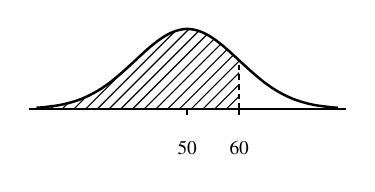
\begin{tikzpicture}[x=0.0127cm, y=-0.0127cm]
\path[shade hatch] (25.2,113) -- plot[smooth] coordinates {(25.2,111.8) (28.6,111.6) (32.1,111.3) (35.5,110.9) (38.9,110.5) (42.4,110.1) (45.8,109.5) (49.3,108.9) (52.7,108.2) (56.1,107.4) (59.6,106.5) (63.0,105.5) (66.4,104.3) (69.9,103.0) (73.3,101.6) (76.8,100.1) (80.2,98.3) (83.6,96.5) (87.1,94.5) (90.5,92.3) (93.9,90.0) (97.4,87.5) (100.8,84.9) (104.3,82.1) (107.7,79.2) (111.1,76.3) (114.6,73.2) (118.0,70.0) (121.4,66.9) (124.9,63.7) (128.3,60.5) (131.8,57.3) (135.2,54.2) (138.6,51.2) (142.1,48.3) (145.5,45.6) (148.9,43.1) (152.4,40.8) (155.8,38.8) (159.3,37.0) (162.7,35.6) (166.1,34.4) (169.6,33.6) (173.0,33.1) (176.4,33.0) (179.9,33.2) (183.3,33.8) (186.8,34.7) (190.2,35.9) (193.6,37.5) (197.1,39.3) (200.5,41.4) (203.9,43.8) (207.4,46.3) (210.8,49.1) (214.3,52.0) (217.7,55.0) (221.1,58.1) (224.6,61.3) (228.0,64.5)} -- (228,113) -- cycle;
\draw (17.2,113) -- (334.8,113);
\draw[line width=0.9pt] plot[smooth] coordinates {(25.2,111.8) (28.6,111.6) (32.0,111.3) (35.4,110.9) (38.8,110.5) (42.1,110.1) (45.5,109.6) (48.9,109.0) (52.3,108.3) (55.7,107.5) (59.1,106.6) (62.5,105.6) (65.9,104.5) (69.3,103.3) (72.6,101.9) (76.0,100.4) (79.4,98.7) (82.8,96.9) (86.2,95.0) (89.6,92.9) (93.0,90.6) (96.4,88.2) (99.8,85.7) (103.1,83.0) (106.5,80.2) (109.9,77.3) (113.3,74.3) (116.7,71.2) (120.1,68.1) (123.5,65.0) (126.9,61.8) (130.3,58.7) (133.6,55.6) (137.0,52.6) (140.4,49.7) (143.8,47.0) (147.2,44.4) (150.6,42.0) (154.0,39.9) (157.4,38.0) (160.8,36.4) (164.1,35.1) (167.5,34.1) (170.9,33.4) (174.3,33.0) (177.7,33.0) (181.1,33.4) (184.5,34.1) (187.9,35.1) (191.2,36.4) (194.6,38.0) (198.0,39.9) (201.4,42.0) (204.8,44.4) (208.2,47.0) (211.6,49.7) (215.0,52.6) (218.4,55.6) (221.7,58.7) (225.1,61.8) (228.5,65.0) (231.9,68.1) (235.3,71.2) (238.7,74.3) (242.1,77.3) (245.5,80.2) (248.9,83.0) (252.2,85.7) (255.6,88.2) (259.0,90.6) (262.4,92.9) (265.8,95.0) (269.2,96.9) (272.6,98.7) (276.0,100.4) (279.4,101.9) (282.7,103.3) (286.1,104.5) (289.5,105.6) (292.9,106.6) (296.3,107.5) (299.7,108.3) (303.1,109.0) (306.5,109.6) (309.9,110.1) (313.2,110.5) (316.6,110.9) (320.0,111.3) (323.4,111.6) (326.8,111.8)};
\draw[aux] (228,113) -- (228,64.5);
\draw (176,113) -- (176,119);
\draw (228,113) -- (228,119);
\node[font=\scriptsize, anchor=north] at (176,135) {$50$};
\node[font=\scriptsize, anchor=north] at (228,135) {$60$};
\end{tikzpicture}
\end{document}
